\documentclass[a4paper,12pt]{article}
\usepackage[slovene]{babel}
\usepackage[utf8]{inputenc}
\usepackage{multicol}
\usepackage{fullpage}
\usepackage{guitar}
\usepackage{titlesec}
\usepackage{graphicx}
\setcounter{secnumdepth}{-1} 
\usepackage[absolute]{textpos}
\titleformat{\chapter}{\large\bfseries}{\thesection}{1em}{}
\titleformat{\section}{\Large\bfseries}{\thesection}{1em}{}
\titleformat{\subsection}{\large\bfseries}{\thesection}{1em}{}

\begin{document}
\pagenumbering{Roman}
\begin{titlepage}
\begin{textblock*}{297mm}(-6mm,-0mm)
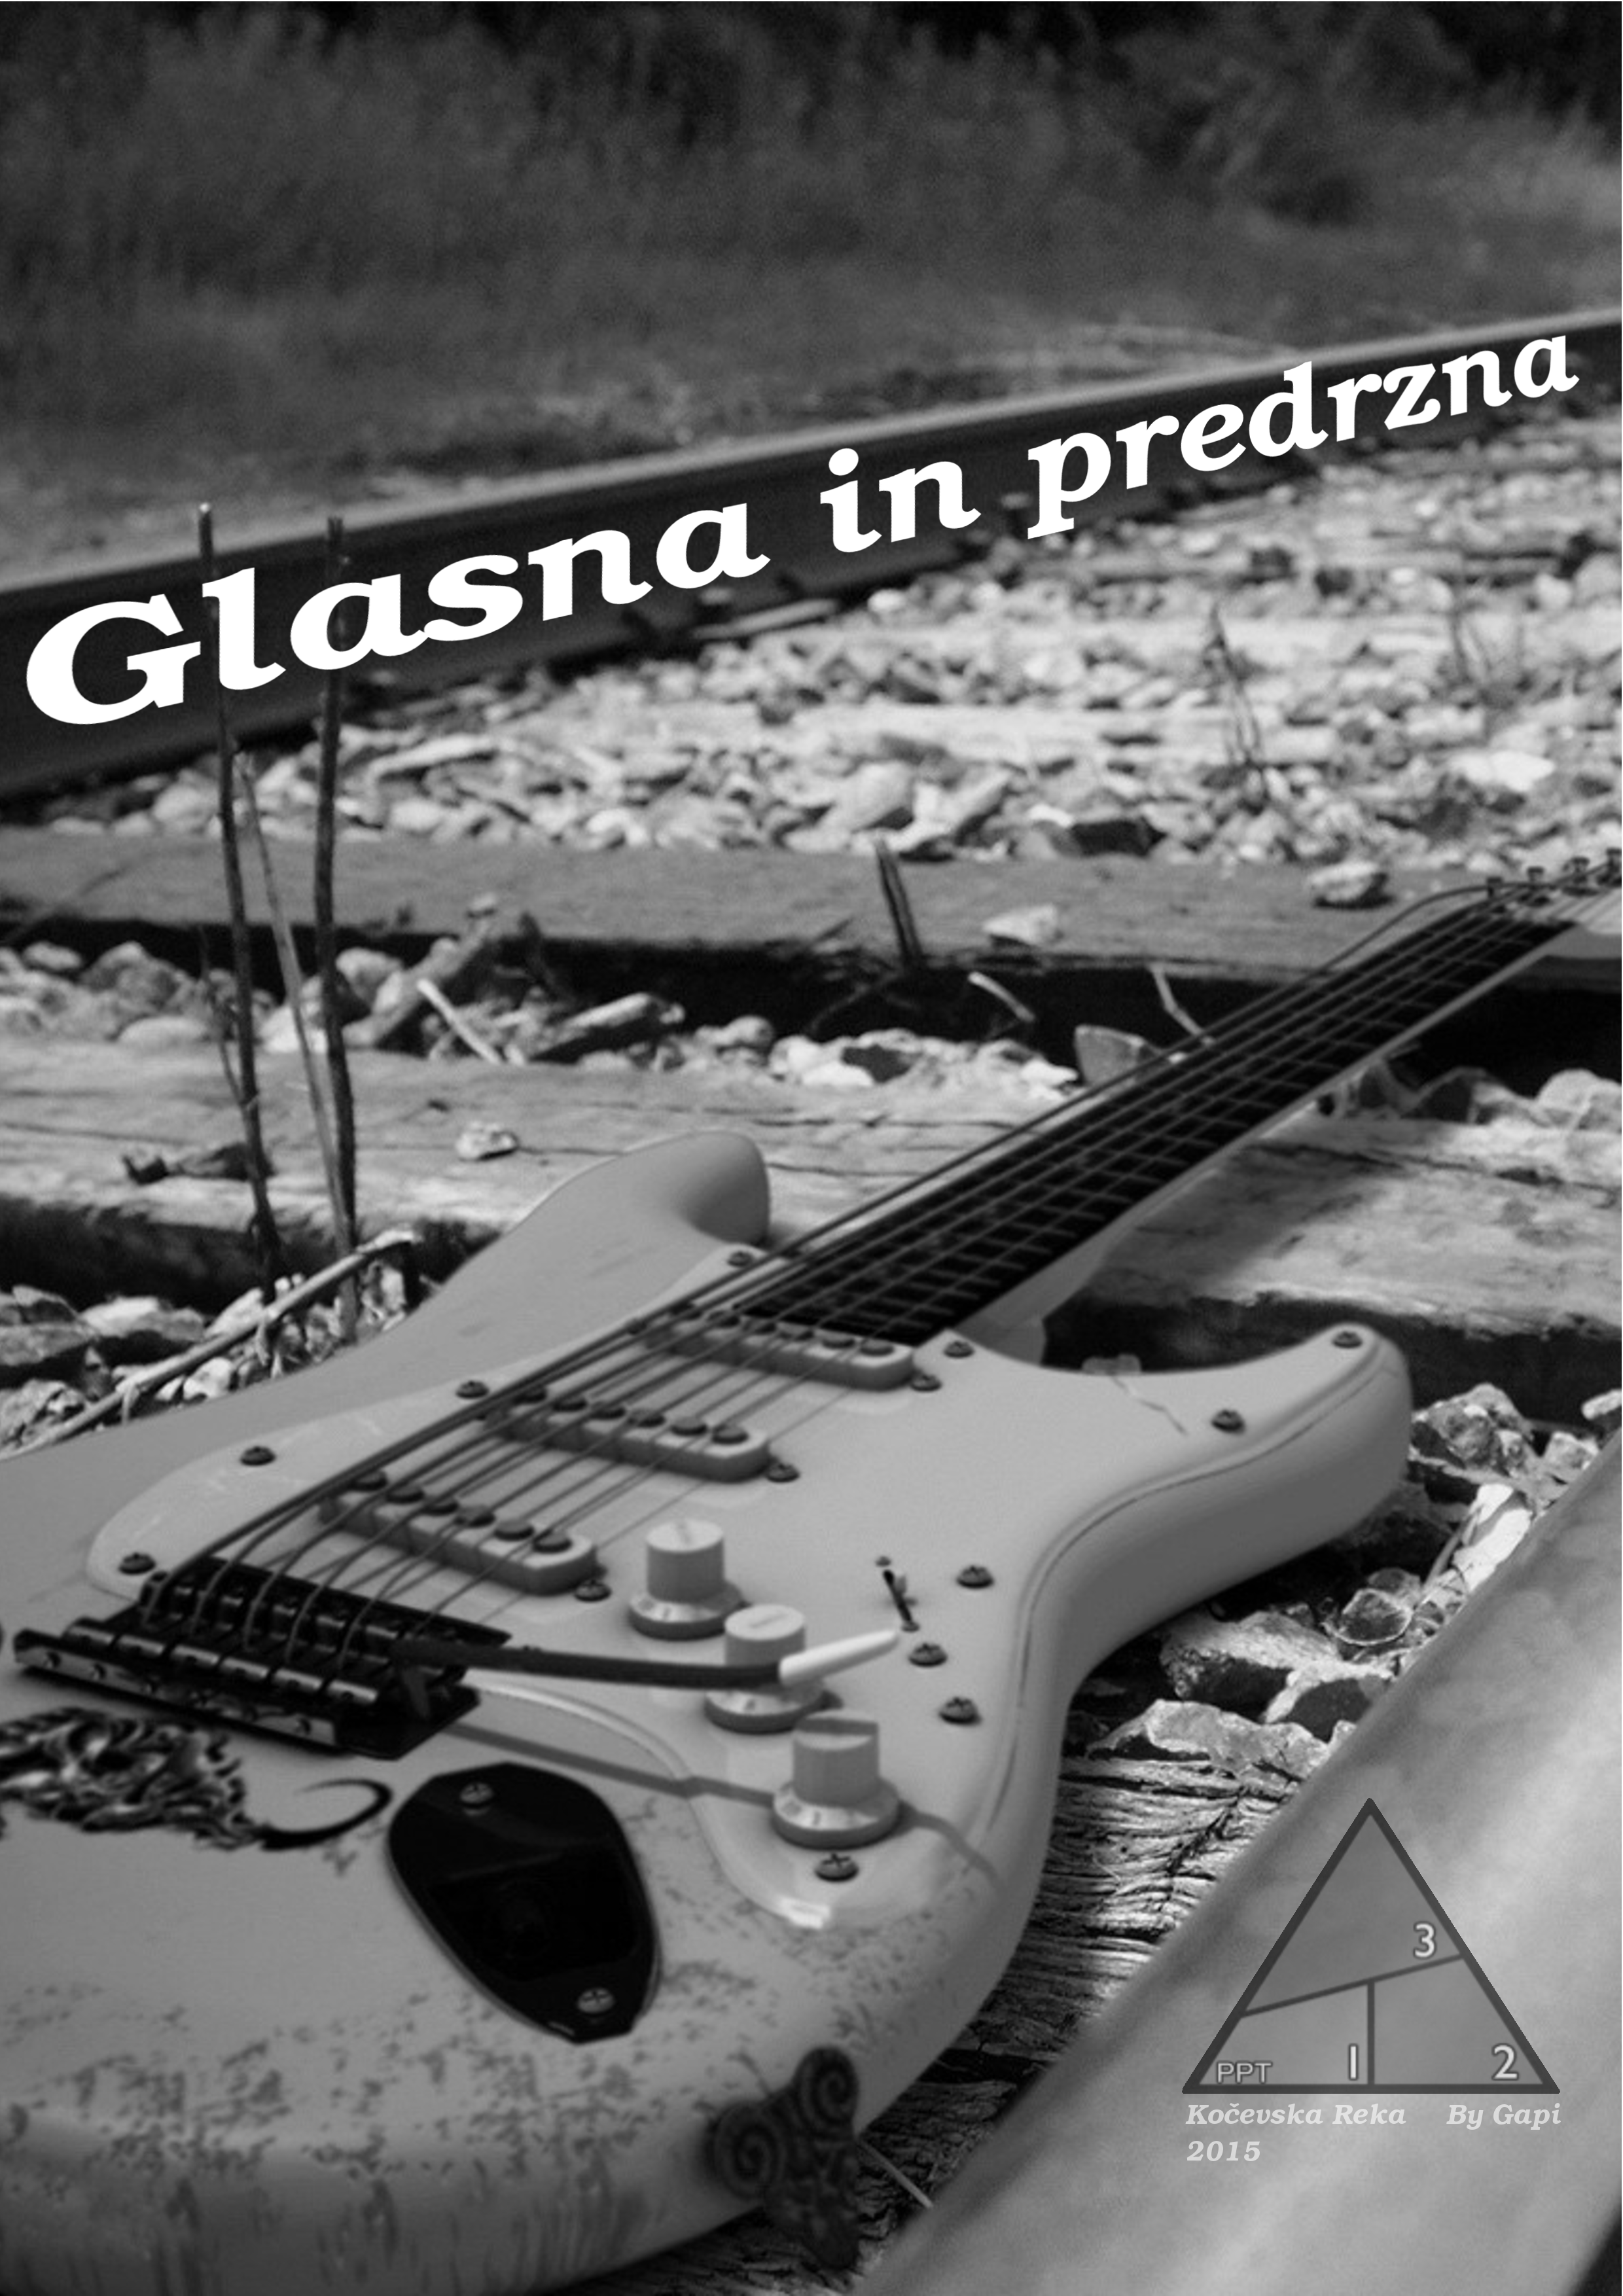
\includegraphics[width=\paperwidth]{img/tpage.png}
\end{textblock*} \
\end{titlepage}
\setlength{\columnseprule}{0.5pt}
\begin{multicols}{2}
\tableofcontents
\end{multicols}
\pagebreak

\setlength{\columnseprule}{0.5pt}
\begin{multicols}{2}
\pagenumbering{arabic}
\section{Akordi}
\begin{guitar}
[A - X02220  Am - X02210]

[B - X13331  Bm - X13321]

[C - X32010  Cm - X35543]  

[D - XX0232  Dm - XX0231] 

[E - 022100  Em - 022000] 

[F - 133211  Fm - 133111]

[G - 320003  Gm - 355333]

[H - X24442  Hm - X24432]


[A7 - X02020  B7 - X13131]

[C7 - X32310  D7 - XX0212]

[E7 - 020100  F7 - 131211]

[G7 - 320001  H7 - X21202]


[Am7 - X02010  Bm7 - X13121]

[Cm7 - X35343  Dm7 - XX0211]

[Em7 - 022030  Fm7 - 131111]

[Gm7 - 353333  Hm7 - X24232]


[C# - X46664  D# - 779997]

[F# - 244322  G# - 466544]


[C#m - X46654  D#m - 779987]

[F#m - 133111  G#m - 466444]


[A6 - X02222  C6 - X055555]

[D6 - X077777 E6 - X099999]


[ASUS2 - X02200]

[ASUS4 - X02230]

[DSUS2 - XX0320] 

[DSUS4 - XX0233]

[ESUS4 - 022200]

[CMAJ7 - X32000]

[FMAJ7 - 103210]

[GMAJ7 - 3X0032]

[DADD4/ADD2 - 554030]

\end{guitar}
\subsection*{Barre akordi}
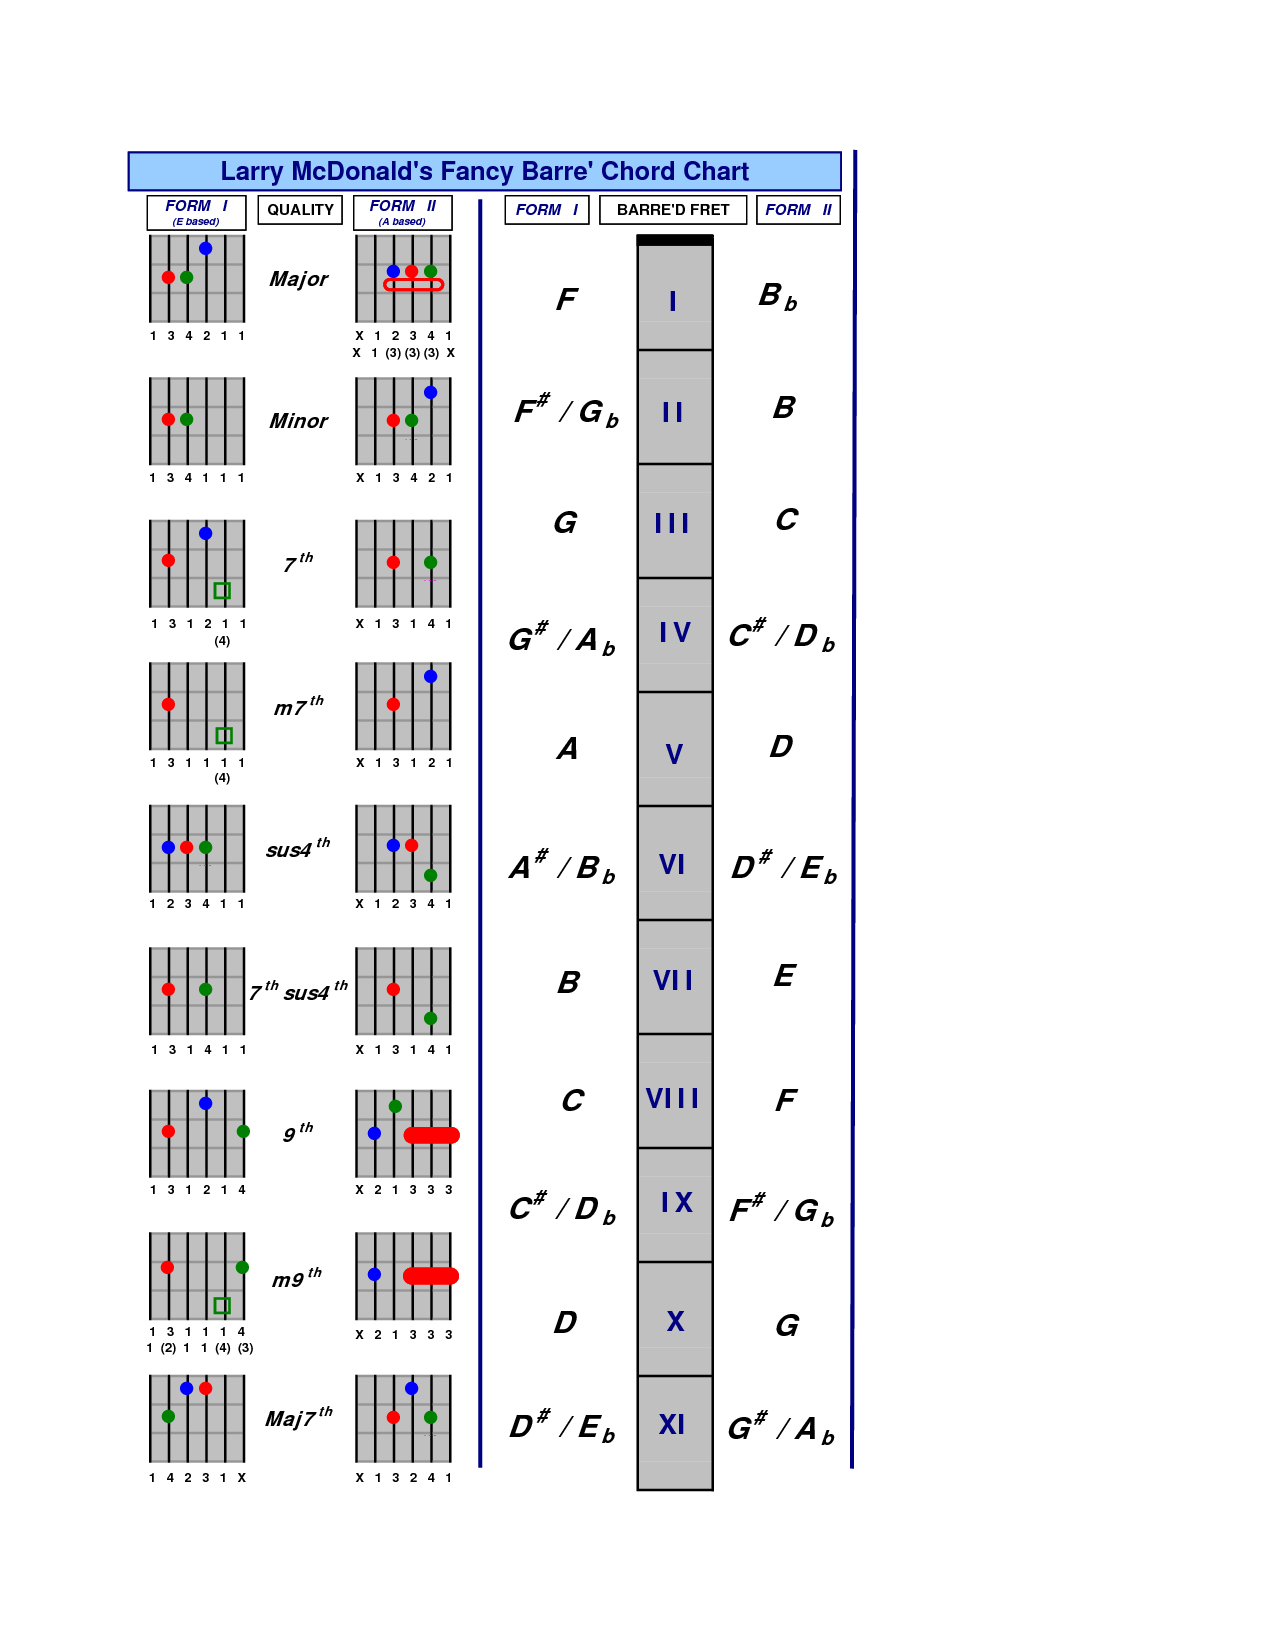
\includegraphics[width=140mm]{img/barre.png}
\clearpage
\section{Krokodilčki}
\subsection*{Čuki}
\begin{guitar}
[D]Modna pista [G]to je [A]prava [D]stvar, [G A]'
[D]lepe punce - [G]te so božji [A]dar, [G A]'
[D]glej jo, glej jo, [G]ta bo [A]miss sve[D]ta, [G A]'
še [D]spat ne morem, [A]ker želim si [D]da:


Njene dolge no[G]ge z mano v [A]stric bi h[D]odile,
le poglej njen nas[G]meh, kroko[A]dilčke v o[D]ceh.
Modna pista ods[G]lej bo po [A]mojih ko[D]lenih,
sam bom čuval nas[G]meh, kroko[A]dilčke v o[D]ceh,
[A]v o[D]ceh!


Sam se zdaj potikam naokrog.
Daleč stran od njenih dolgih nog.
Daleč stran od modnega sveta,
vendar si želim še vedno da:


Njene dolge noge...   

\end{guitar}
\section{Lovro}
\subsection*{Big foot mama}
\begin{guitar}
[C Am Em G] 

[C]Caku je Lovro, [Am]caku vsak dan.
[Em]Caku je nevesto, [G]sovražu je bit sam.
[C]Zeleu si je vsaj enkrat ji [Am]modrček odpet,
[Em]saj mu brez nje tko [G]več ni blo za žvet.


In zvezde so sijale, gor na njen balkon,
a on je kr naenkrat zavrtu telefon.


[F]Rad bi biu s tabo [G]in bi se smeju spet,
[Am]ne da se mi več tok trpet,
[Am]ne da se mi več tok trpet.
[F]Rad bi biu s tabo [G]in bi se smeju spet,
[C]hočem te za sebe met,
[C]O hočem te za sebe met.

[C Am Em G] 

Že naslednjo noč ni preživu sam, 
predala sta se strasti,
nobenga ni blo sram.


A sreča ni bla dolga, pismo je pršlo,
bila je zaročena, nesla ga je okrog.


In nč mu ni blo jasn, 
le blo mu je hudo, 
za to noč bil je dobr, 
za več pa bl težko.


Rad bi bil s tabo...
 
[C Am Em G C Am]

Čaku je spet Lovro, čaku vsak dan.
Dočaku ni neveste, niti beli dan.
Napisu je le pismo in še njen naslov,
na vrtzu se je obesu, v smrt se je pognou. 

                         
[F]Ceprov bi rajš bil s tabo 
[G]in bi se smeju spet.
[C]Nism mogu več trpet,
O nism mogu več trpet.


Rajš bi bil s tabo... (2x)

\end{guitar}
\section{What's up?}
\subsection*{4 Non Blondes}
\begin{guitar}
[G]Twenty Five years and my life stood still
[Am]Trying to get up that 
great big hill of [C]hope
For a desti[G]nation


I realized quickly when I knew that I should
That the world was made of this 
brotherhood of man
For whatever that means

                                   
[G]And So I cry sometimes 
when I'm lying in bed
Just to [Am]get it all out
whats in my head and I, 
[C]I am feeling a little pe[G]culiar.

 
So I wake in the morning 
and I step outside
and I take a deep breath 
and I get real high and
I Scream at the top of my lungs 
WHATS GOIN ON?


[G]And I said Heyeyeyeyey 
[Am]Heyeyey
I said [C]Hey Whats going [G]on?
[G]And I said Heyeyeyeyey
[Am]Heyeyey
I said [C]Hey Whats going [G]on?


And I [G]try, oh my god do I [Am]try
I try all the [C]time, in this insti[G]tution
And I pray, oh my god do I pray
I pray every single day
For a revolution

               
And So I cry sometimes...


Twenty-five years and my life stood still
Trying to get up that great big hill of hope
For a destination...


\end{guitar}
\end{multicols}
\clearpage
\clearpage
\null
\vfill
\center

\includegraphics[width=100px]{img/licence.png}

Pesmarica je zaščitena z licenco CC-BY-NC-SA. Vse pesmi so delo in last avtorjev. Morebitne napake in predloge sporočite na pesmarica.info@gmail.com 

Izvorna koda (LaTeX) ter PDF sta dostopna na https://github.com/gztproject/Pesmarica
\end{document}
